% Copyright (C) 2012 by Paul Gaborit
%
% This file may be distributed and/or modified
%
% 1. under the LaTeX Project Public License and/or
% 2. under the GNU Public License.

\documentclass[11pt,hyperref={colorlinks=false,runcolor=blue}]{beamer}
%\usetheme{Warsaw}
\usepackage[T1]{fontenc}
\usepackage{lmodern}
\usepackage{tikz}
\usetikzlibrary{backgrounds,fit,calc,shadows,chains,ocgx,shapes.geometric}
\usepackage{microtype}
\usepackage{url}
\usepackage{fancyvrb}
\usepackage{listings}
\lstdefinestyle{TeXcode}{
  fancyvrb=true,
  language=[LaTeX]TeX,
  basicstyle=\scriptsize\ttfamily,
  keywordstyle=\color{blue}\bfseries,
  commentstyle=\color{red!50!black}\itshape,
  stringstyle=\ttfamily\color{green!50!black},
  showspaces=false,
  showstringspaces=false,
  backgroundcolor=\color{white},
  fontadjust=true,
  aboveskip=1ex,
  belowskip=1ex,
  emphstyle=\color{blue}\bfseries,
  keepspaces=true,
  flexiblecolumns=true,
  emph={switchocg,showocg,hideocg,actionsocg,usetikzlibrary}
}
\newcommand\TkzTileWallPaper[3]{
  \pgfmathtruncatemacro{\nx}{\paperwidth/#1}
  \foreach \dx in {0,...,\nx}{
    \pgfmathtruncatemacro{\ny}{\paperheight/#2}
    \foreach \dy in {0,...,\ny}{
      \node[anchor=south west,inner sep=0pt]
      at ([xshift=#1 * \dx,yshift=#2 * \dy]current page.south west)
      {\includegraphics[width=#1,height=#2]{#3}};
    }
  }
}

\setbeamersize{text margin left=3mm,text margin right=3mm}

\newcommand\latex{{\rmfamily\LaTeX}}

\newcommand{\TikZ}{Ti\emph{k}Z}

\begin{document}
\begin{frame}[fragile]
  \frametitle{\latex{}, OCG \& \TikZ{}  (without JavaScript): \texttt{ocgx} package}
  \framesubtitle{by Paul \textsc{Gaborit} wiht help of Paul
    \textsc{Isambert}}

  \begin{alertblock}{PDF readers}
    To fully enjoy this demonstration, use \emph{Adobe Reader},
    \emph{Foxit Reader} or \emph{evince}!
  \end{alertblock}

  \begin{columns}

    \column{.6\linewidth}

    \begin{block}{Simple example: code}
    \begin{lstlisting}[style=TeXcode]
\begin{ocg}{My first OCG}{refmyfirstocg}{1}
   Some content...
\end{ocg}

\switchocg{refmyfirstocg}%
{\textcolor{red}{Click me!}}
\end{lstlisting}
    \end{block}

    \column{.4\linewidth}
    
    \begin{block}{Simple example: result}
      
      \begin{ocg}{My first OCG}{refmyfirstocg}{1}
        Some content...
      \end{ocg}
      
      \switchocg{refmyfirstocg}%
      {\textcolor{red}{Click me!}}
      
    \end{block}
  \end{columns}

\end{frame}

\begin{frame}
  \frametitle{First example with Ti\emph{k}Z}
  
  {\centering
  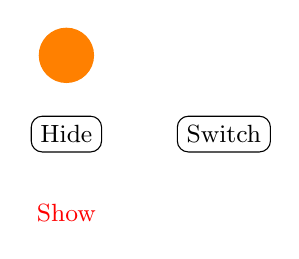
\begin{tikzpicture}[font=\small]
    \begin{scope}[ocg={ref=toto,status=visible,name=ok}]
      \fill[orange] circle(10pt);
      \node[draw,rounded corners,hide ocg=toto] at (0,-1) {Hide};
      \node[draw,rounded corners,switch ocg=toto] at (2,-1) {Switch};
    \end{scope}
    \node[show ocg=toto,text=red] at (0,-2) {Show};
  \end{tikzpicture}\par}

  \begin{itemize}
  \item \switchocg{toto}{\Large \textcolor{red}{A very long phrase to
        show that a link can be on multiple lines\ldots}\par\textcolor{red}{And with two
        paragraphs!}}
  \item The ``Switch'' button is \textbf{always} useable!
  \end{itemize}
\end{frame}

\tikzset{%
  button on/.style={%
    draw,circle,drop shadow,
    line width=1pt,
    fill=lime!50,
    switch ocg with mark on={#1}{},
  },
}
\begin{frame}
  \frametitle{An ordered stack}
  
  \centering
  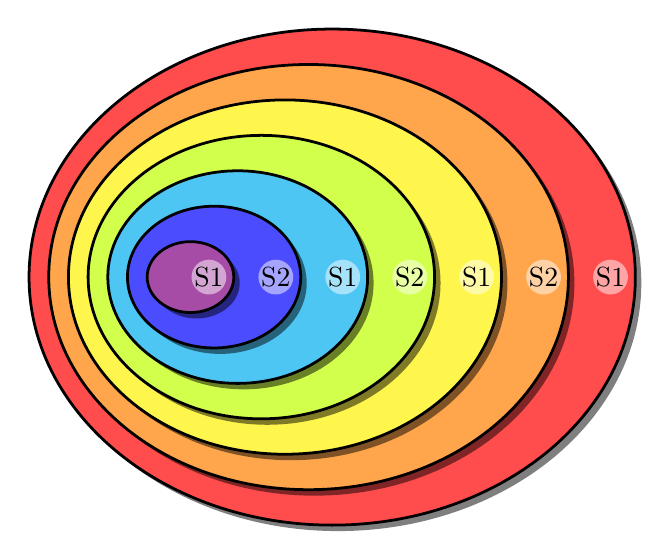
\begin{tikzpicture}
    \foreach \col[count=\c] in {red,orange,yellow,lime,cyan,blue,violet}{
      \pgfmathtruncatemacro{\num}{mod(\c+1,2)+1}
      \pgfmathsetmacro{\rad}{8-\c}
      \begin{scope}[xshift=-.3*\c cm,ocg={name=s\num,ref=s\num}]
        \node[ellipse,draw,line width=1pt,
        minimum width=1.1*\rad cm,minimum height=.9*\rad cm,
        fill=\col!70,drop shadow={fill=black}](t){};
        \node[left=3pt of t.east,fill=white,
        fill opacity=.5,text opacity=1,circle,inner sep=0pt]{S\num};
      \end{scope}
    }
  \end{tikzpicture}

  \begin{tikzpicture}
    \node[button on=s1](but){};
    \node[right=0 of but]{Switch S1};
    \node[below=3pt of but,button on=s2](but){};
    \node[right=0 of but]{Switch S2};
  \end{tikzpicture}

\end{frame}

\begin{frame}
  \frametitle{RGB and CMY color models with \texttt{xcolor}}

  \def\mylist{red/0,yellow/60,green/120,cyan/180,blue/240,magenta/300}
  \centering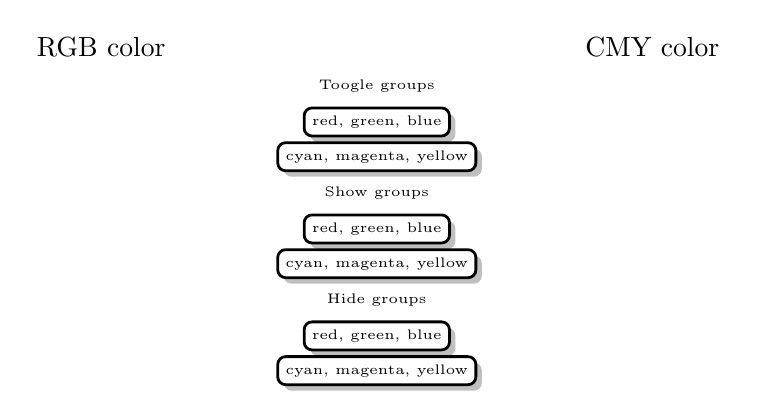
\begin{tikzpicture}[line width=1pt]
    \begin{scope}
      \node at (90:25mm) {RGB color};
      \foreach \col/\angle in \mylist {
        \colorlet{rgb \col}[rgb]{\col}
        \draw  (\angle:5mm) circle [radius=10mm];
        \begin{scope}[on background layer]
          \begin{scope}[ocg={ref=RGB\col,name=RGB \col}]
            \fill[fill=rgb \col,fill opacity=.5]
            (\angle:5mm) circle [radius=10mm];
          \end{scope}
        \end{scope}
        
        \node[rounded corners=1mm,draw,line width=1pt,
        minimum size=3mm,fill=rgb \col,fill opacity=.5,
        drop shadow,
        inner sep=0,inner xsep=0,
        switch ocg with mark on={RGB\col}{}]
        at (\angle:20mm){};
      }
    \end{scope}
    \begin{scope}[xshift=70mm]
      \node at (90:25mm) {CMY color};
      \foreach \col/\angle in \mylist {
        \colorlet{cmy \col}[cmyk]{\col}
        \draw  (\angle:5mm) circle [radius=10mm];
        \begin{scope}[on background layer]
          \begin{scope}[ocg={ref=CMY\col,name=CMY \col}]
            \fill[fill=cmy \col,fill opacity=.5]
            (\angle:5mm) circle [radius=10mm];
          \end{scope}
        \end{scope}
      
        \node[rounded corners=1mm,draw,line width=1pt,
        minimum size=3mm,fill=cmy \col,fill opacity=.5,
        drop shadow,inner sep=0,outer sep=0,
        switch ocg with mark on={CMY\col}{}]
        at (\angle:20mm){};
      }
    \end{scope}
    
    \begin{scope}%
      [xshift=35mm,start chain=going below,node distance=.5mm,font=\tiny]
      \node[on chain] at (0,20mm) {Toogle groups};
      \node%
      [on chain,draw,rounded corners=1mm,fill=white,drop shadow,
      minimum size=3mm,inner sep=1mm,
      switch ocg={RGBred RGBblue RGBgreen CMYred CMYblue CMYgreen},
      ]
      {red, green, blue};
      \node%
      [on chain,draw,rounded corners=1mm,fill=white,drop shadow,
      minimum size=3mm,inner sep=1mm,
      switch ocg={RGByellow RGBcyan RGBmagenta CMYyellow CMYcyan CMYmagenta},
      ]
      {cyan, magenta, yellow};
      
      \node[on chain] {Show groups};
      \node%
      [on chain,draw,rounded corners=1mm,fill=white,drop shadow,
      minimum size=3mm,inner sep=1mm,
      show ocg={RGBred RGBblue RGBgreen CMYred CMYblue CMYgreen},
      ]
      {red, green, blue};
      \node%
      [on chain,draw,rounded corners=1mm,fill=white,drop shadow,
      minimum size=3mm,inner sep=1mm,
      show ocg={RGByellow RGBcyan RGBmagenta CMYyellow CMYcyan CMYmagenta},
      ]
      {cyan, magenta, yellow};

      \node[on chain] {Hide groups};
      \node%
      [on chain,draw,rounded corners=1mm,fill=white,drop shadow,
      minimum size=3mm,inner sep=1mm,
      hide ocg={RGBred RGBblue RGBgreen CMYred CMYblue CMYgreen},
      ]
      {red, green, blue};
      \node%
      [on chain,draw,rounded corners=1mm,fill=white,drop shadow,
      minimum size=3mm,inner sep=1mm,
      hide ocg={RGByellow RGBcyan RGBmagenta CMYyellow CMYcyan CMYmagenta},
      ]
      {cyan, magenta, yellow};
    \end{scope}
    
  \end{tikzpicture}\par

\end{frame}

\foreach \name/\link/\ltxlink/\tiles in {%
  The Big Show/%
  {http://designfestival.com/the-cicada-principle-and-why-it-matters-to-web-designers/}/%
  {http://latex-community.org/know-how/433-tiled-backgrounds}/%
  {%
    curtain1/32.7pt/\paperheight,%
    curtain2/90pt/\paperheight,%
    curtain3/210.9pt/\paperheight%
  },%
  Mosaic/%
  {http://designfestival.com/cicada/break-it-down/?id=95}/%
  {http://latex-community.org/know-how/433-tiled-backgrounds}/%
  {%
    mosaic1/30pt/30pt,%
    mosaic2/70pt/70pt,%
    mosaic3/110pt/110pt,%
    mosaic4/110pt/110pt%
  }%
}{
  \begin{frame}
    \begin{tikzpicture}[remember picture,overlay]
      \foreach \pictname/\wid/\hei in \tiles {
        \begin{scope}[ocg={name=\pictname,ref=\pictname}]
          \TkzTileWallPaper{\wid}{\hei}{\pictname}
        \end{scope}
      }

    \end{tikzpicture}
    
    \centering
\begin{tikzpicture}[start chain=going below,node distance=1em]
      \node[fill=white,fill opacity=.75,align=center,
      text=black,font=\tiny\bfseries,text opacity=1,
      on chain,
      rounded corners=2mm]
      {{\huge\name}\\\url{\link}\\(\latex{} \url{\ltxlink})};

      \foreach \pictname/\wid/\hei in \tiles {

        \node[on chain,text=white,fill=black,fill opacity=.5,text opacity=1,
        text width=3cm,align=center,font=\bfseries]
        (a) {\hspace{5mm}\pictname};

        \node[rounded corners=1mm,draw,line width=1pt,%
        minimum size=3mm,top color=white,bottom color=black,
        fill opacity=.5,
        drop shadow={fill=black},
        switch ocg with mark on={\pictname}{}]
        at ([xshift=3mm,yshift=.5mm]a.west) {};
        
      }
    \end{tikzpicture}\par
  \end{frame}
}

\begin{frame}
  \frametitle{Microtype demo (first version without hierarchy)}

  \def\sampletext{%
    Margin kerning is the adjustments of the characters at the
    margins of a typeset text.  A simplified employment of margin
    kerning is hanging punctuation. Margin kerning is needed for
    optical alignment of the margins of a typeset text, because
    mechanical justification of the margins makes them look rather
    ragged. Some characters can make a line appear shorter to the
    human eye than others. Shifting such characters by an
    appropriate amount into the margins would greatly improve the
    appearance of a typeset text.%
  }

  \tikzset{
    checkbox/.style={
      draw,circle,line width=.5pt,%
      minimum size=.5em,top color=white,bottom color=cyan,
      fill opacity=1,
      inner sep=0,
      drop shadow={fill=black,shadow xshift=.5mm,shadow yshift=-.5mm},
    },
    sampletext/.style={
      text width=8cm,align=justify,
      font=\small,
      fill=yellow!20,
      inner xsep=1.5cm,
      inner ysep=1cm,
      draw=gray,
    },
  }

  {\centering
    \begin{tikzpicture}
      \begin{scope}[ocg={name=With Protrusion,ref=protrusion}]        
      \end{scope}
      \begin{scope}[ocg={name=Without Protrusion,ref=no-protrusion,status=invisible}]        
      \end{scope}
      \begin{scope}[ocg={name=With Expansion,ref=expansion}]        
      \end{scope}
      \begin{scope}[ocg={name=With Protrusion,ref=protrusion}]        
      \end{scope}
      \begin{scope}[ocg={name=Without Expansion,ref=no-expansion,status=invisible}]        
      \end{scope}
      \begin{scope}[ocg={name=With Protrusion,ref=protrusion}]
        \microtypesetup{protrusion=true}%
        \begin{scope}[ocg={name=With Expansion,ref=expansion}]
          \microtypesetup{expansion=true}%
          \node[sampletext]{\sampletext\par};%
        \end{scope}
        
        \begin{scope}[ocg={name=Without Expansion,status=invisible,ref=no-expansion}]
          \microtypesetup{expansion=false}%
          \node[sampletext]{\sampletext\par};%
        \end{scope}
      \end{scope}
      
      \begin{scope}[ocg={name=Without Protrusion,status=invisible,ref=no-protrusion}]
        \microtypesetup{protrusion=false}%
        \begin{scope}[ocg={name=With Expansion,ref=expansion}]
          \microtypesetup{expansion=true}%
          \node[sampletext]{\sampletext\par};%
        \end{scope}
        
        \begin{scope}[ocg={name=Without Expansion,status=invisible,ref=no-expansion}]
          \microtypesetup{expansion=false}%
          \node[sampletext]{\sampletext\par};%
        \end{scope}
      \end{scope}
    \end{tikzpicture}\par
  }

  Microtype :
  \begin{tikzpicture}
    \node[checkbox,switch ocg with mark on={protrusion}{no-protrusion}]{};
  \end{tikzpicture} with protrusion 
  \begin{tikzpicture}
    \node[checkbox,switch ocg with mark on={expansion}{no-expansion}]{};
  \end{tikzpicture} with expansion
  
\end{frame}

\begin{frame}
  \frametitle{Microtype demo (second version with hierarchy)}

  \def\sampletext{%
    Margin kerning is the adjustments of the characters at the
    margins of a typeset text.  A simplified employment of margin
    kerning is hanging punctuation. Margin kerning is needed for
    optical alignment of the margins of a typeset text, because
    mechanical justification of the margins makes them look rather
    ragged. Some characters can make a line appear shorter to the
    human eye than others. Shifting such characters by an
    appropriate amount into the margins would greatly improve the
    appearance of a typeset text.%
  }

  \tikzset{
    checkbox/.style={
      draw,circle,line width=.5pt,%
      minimum size=.5em,top color=white,bottom color=cyan,
      fill opacity=1,
      inner sep=0,
      drop shadow={fill=black,shadow xshift=.5mm,shadow yshift=-.5mm},
    },
    sampletext/.style={
      text width=8cm,align=justify,
      font=\small,
      fill=yellow!20,
      inner xsep=1.5cm,
      inner ysep=1cm,
      draw=gray,
    },
  }

  {\centering
    \begin{tikzpicture}
      \begin{scope}[ocg={name=With Protrusion,ref=pro}]
        \microtypesetup{protrusion=true}%
        \begin{scope}[ocg={name=With Expansion,status=visible,ref=pro-exp}]
          \microtypesetup{expansion=true}%
          \node[sampletext]{\sampletext\par};%
        \end{scope}
        
        \begin{scope}[ocg={name=Without Expansion,status=invisible,ref=pro-no-exp}]
          \microtypesetup{expansion=false}%
          \node[sampletext]{\sampletext\par};%
        \end{scope}
      \end{scope}
      
      \begin{scope}[ocg={name=Without Protrusion,status=invisible,ref=no-pro}]
        \microtypesetup{protrusion=false}%
        \begin{scope}[ocg={name=With Expansion,status=visible,ref=no-pro-exp}]
          \microtypesetup{expansion=true}%
          \node[sampletext]{\sampletext\par};%
        \end{scope}
        
        \begin{scope}[ocg={name=Without Expansion,status=invisible,ref=no-pro-no-exp}]
          \microtypesetup{expansion=false}%
          \node[sampletext]{\sampletext\par};%
        \end{scope}
      \end{scope}
    \end{tikzpicture}\par
  }

  Microtype :
  \begin{tikzpicture}
    \node[checkbox,switch ocg with mark on={pro}{no-pro}]{};
  \end{tikzpicture} with protrusion 
  \begin{tikzpicture}
    \node[checkbox,switch ocg with mark on={pro-exp}{pro-no-exp no-pro-exp no-pro-no-exp}]{};
  \end{tikzpicture} with expansion
  
\end{frame}
\end{document}

%%% Local Variables: 
%%% mode: latex
%%% TeX-master: t
%%% End: 
